\documentclass{article}

\usepackage{tikz}
\usetikzlibrary{patterns}
\usetikzlibrary{scopes}
\begin{document}

\def\iangle{35} % Angle of the inclined plane

\def\down{-90}
\def\arcr{0.5cm} % Radius of the arc used to indicate angles

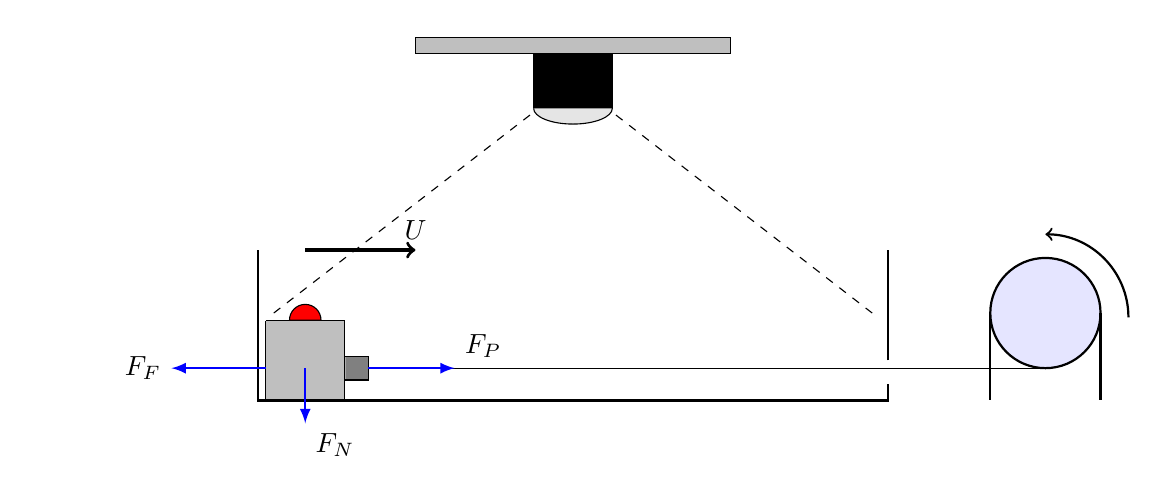
\begin{tikzpicture}[
    force/.style={>=latex, thick, draw=blue,fill=blue},
    axis/.style={densely dashed,gray,font=\small},
    M/.style={rectangle,draw,fill=lightgray,minimum size=0.5cm,thin},
    m/.style={rectangle,draw=black,fill=lightgray,minimum size=0.3cm,thin},
    plane/.style={draw=black,fill=blue!10},
    box/.style={draw=black,fill=lightgray},
    loadcell/.style={draw=black,fill=gray},
    string/.style={draw=red, thick},
    pulley/.style={thick},
    light/.style={draw=black,fill=red},
    camera/.style={draw=black,fill=black},
    lense/.style={draw=black,fill=gray!20},
]

\matrix[column sep=1cm] {

&
% channel
\draw [thick] (0,2) coordinate (base) -- (0,0.09) -- (8,0.09) -- (8,0.3);
\draw [thick] (8, 0.6) -- (8, 2);
% slider
\draw[box] (0.1, 1.1) -- (0.1, 0.1) -- (1.1, 0.1) -- (1.1, 1.1) -- (0.1, 1.1);
% draw load cell
\draw[loadcell]  (1.11, 0.35) -- (1.11, 0.35) -- (1.4, 0.35) -- (1.4, 0.65) -- (1.11, 0.65);
% winch
\draw[plane, thick] (10,1.2) circle [radius=0.7];
\draw [thick] (9.3, 1.2) -- (9.3,0.09);
\draw [thick] (10.7, 1.2) -- (10.7,0.09);
% rope
\draw (1.4, 0.5) -- (10, 0.5);
% light emitting diode
\draw[light] (0.4, 1.11) -- (0.8,1.11) arc(0:180:0.2) --cycle;
% camera
\draw[camera] (3.5, 3.8) -- (4.5, 3.8) -- (4.5, 4.5) -- (3.5, 4.5) -- (3.5, 3.8);
\draw[box] (2, 4.5) -- (6, 4.5) -- (6, 4.7) -- (2, 4.7) -- (2, 4.5);
\draw[lense] (3.5,3.8) arc (180:360:0.5cm and 0.2 cm);
% draw line showing camera field of view
\draw[dashed] (0.2, 1.2) -- (3.5,3.75);
\draw[dashed] (7.8, 1.2) -- (4.5,3.75);
% draw arc
\draw [<-, thick] (10,2.2) arc (90:-0:30pt);
\draw [->, very thick] (0.6, 2) -- (2, 2) node[above]{$U$};
{[force,->]
    % Assuming that Mg = 1. The normal force will therefore be cos(alpha)
    \draw (1.4, 0.5) -- (2.5, 0.5) node[above right] {$F_P$};
    \draw (0.6, 0.5) -- (0.6, -0.2) node[below right] {$F_N$};
    \draw (0.1, 0.5) -- (-1.1, 0.5) node[left] {$F_F$};

}

\\
};
\end{tikzpicture}

\end{document}
